\documentclass[../../Report.tex]{subfiles}
\graphicspath{{\subfix{../../images/}}}
\begin{document}
    In this project, two different samples have been synthesized using two different methods and were investigated 
    for potential use in thermoluminescence dosimetry.\textit{Lithium metasilicate ($Li_2SiO_3$)} 
    was synthesized as the first sample due to its relevance to dosimetry as a tissue equivalent material. The sample 
    was synthesized using solid-state reaction method and dose response was taken. The sample was then doped with
    various rare-earth metals and investigated for optimum doping material.\textit{Calcium Sodium Sulphate ($CaNa_2{(SO_4)}_2$)} was 
    synthesized as our next sample using chemical co-precipitation method.The sample was then doped with Europium at various 
    concentrations and its glow curves were taken.TL glow curves at multiple doses were taken to investigate its dose response. 
    
    \subsection{\large Lithium metasilicate ($Li_2SiO_3$)}
        \subfile{subsections/liso}

    \subsection{\large Calcium Sodium Sulphate ($CaNa_2{(SO_4)}_2$)}
        \subfile{subsections/cana}

    
    \newpage
    \subsection{\large Evaluation of Glow Curves}
        \subfile{subsections/dose}
        
    \subsection{\large Ion Beam Irradiation}
    Calcium Sodium Sulphate ($CaNa_2{(SO_4)}_2$) was irradiated with carbon beams at Inter-University Accelerator
    Centre (IUAC) at two energies 65MeV and 85MeV at different fluences. The samples were first made into pellets using
    a hydraulic pellet press (shown in figure\ref{fig:beam1}). The pellets were then annealed at $400^{\circ}C$ (shown in figure\ref{fig:beam3}) 
    for 2 hours. The samples were then loaded into a ladder (shown in figure\ref{fig:beam2}) and then irradiated using carbon beams from
    pelletron accelerator at IUAC (shown in figure\ref{fig:beam4}). Glow curves were then taken and further analysis was conducted.
    \FloatBarrier\begin{multicols}{2}
        \begin{Figure}
            \centering
            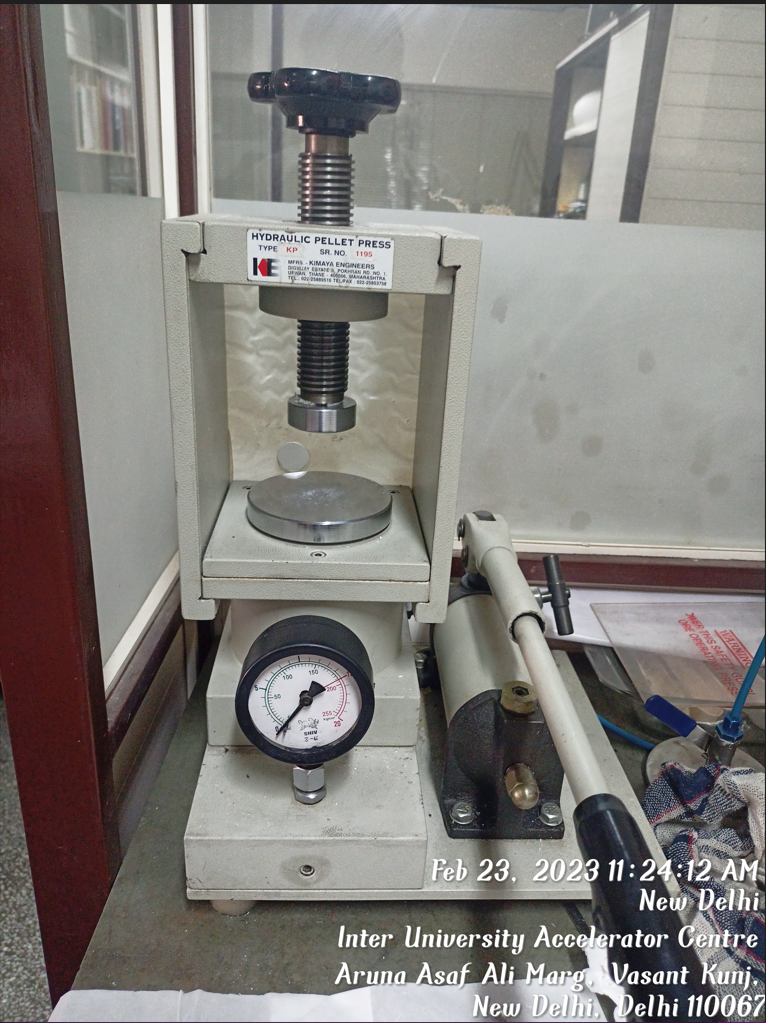
\includegraphics[width=0.6\linewidth]{beam1.png}
            \captionof{figure}{Hydraulic Pellet press to turn the samples into pellets}\label{fig:beam1}
        \end{Figure}
        \begin{Figure}
            \centering
            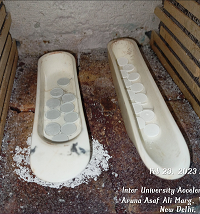
\includegraphics[width=0.6\linewidth]{beam2.png}
            \captionof{figure}{Pellets kept in a boat to be annealed in a muffle furnace}\label{fig:beam2}
        \end{Figure}
    \end{multicols} 
    \pagebreak
    \FloatBarrier\begin{multicols}{2}
        \begin{Figure}
            \centering
            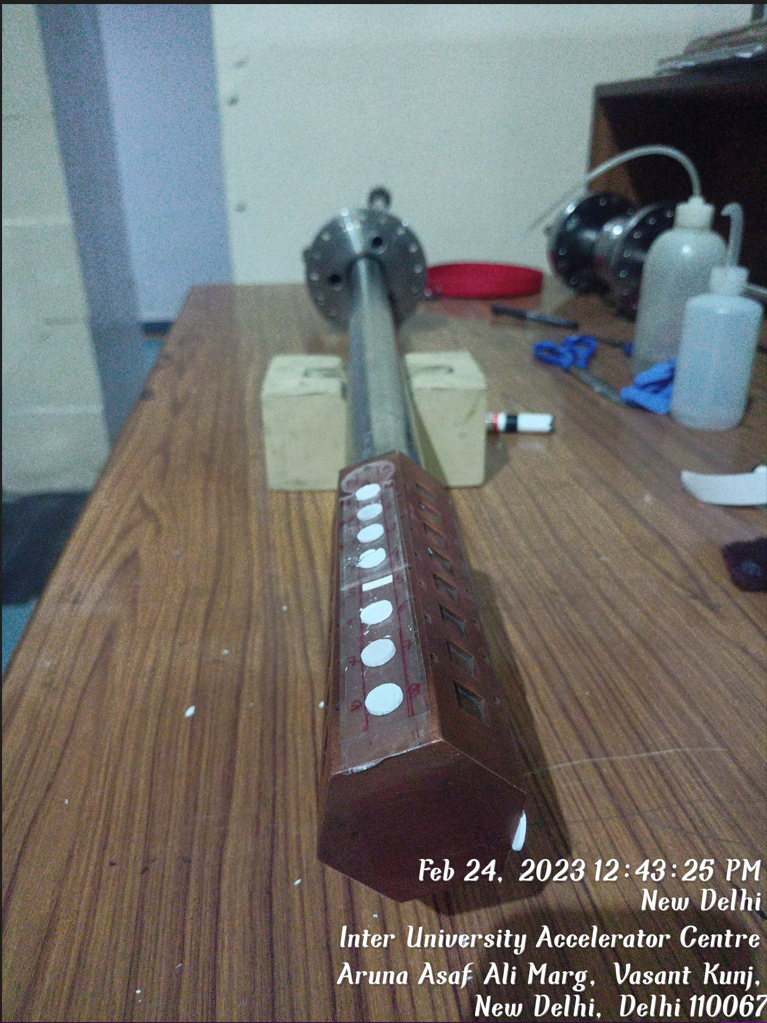
\includegraphics[width=0.6\linewidth]{beam3.png}
            \captionof{figure}{Samples being loaded in a ladder}\label{fig:beam3}
        \end{Figure}
        \begin{Figure}
            \centering
            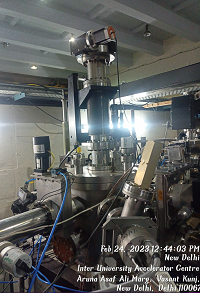
\includegraphics[width=0.6\linewidth]{beam4.png}
            \captionof{figure}{Ion beam irradiation chamber at IUAC}\label{fig:beam4}
        \end{Figure}
    \end{multicols}

    \subsection{\large Deconvolution of TL Glow Curves}
        Deconvolution of a glow curve refers to the process of separating individual glow peaks from a 
        thermoluminescence (TL)\cite{a15} or optically stimulated luminescence (OSL) signal. Glow curves are typically 
        obtained by heating a dosimeter material or stimulating it with light and measuring the emitted 
        luminescence as a function of temperature or time, respectively. Each peak in the glow curve corresponds 
        to a specific trap level in the material, and deconvolution allows the identification and characterization
        of these traps.

        R programming language was used to deconvolute the glow curves obtained using package tgcd\cite{a16}. A code 
        snippet for the R programme used for deconvolution is given below:
        \begin{Figure}
            \centering
            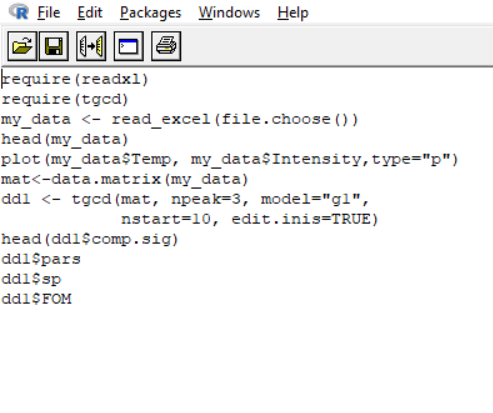
\includegraphics[width=0.8\linewidth]{r.png}
            \captionof{figure}{Code snippet of R program for deconcvolution of glow curves}\label{fig:beam3}
        \end{Figure}
\end{document}